%%%%%%%%%%%%%%%%%%%%%%%%%%%%% Define Article %%%%%%%%%%%%%%%%%%%%%%%%%%%%%%%%%%
\documentclass[11pt]{article}
%%%%%%%%%%%%%%%%%%%%%%%%%%%%%%%%%%%%%%%%%%%%%%%%%%%%%%%%%%%%%%%%%%%%%%%%%%%%%%%

%%%%%%%%%%%%%%%%%%%%%%%%%%%%% Using Packages %%%%%%%%%%%%%%%%%%%%%%%%%%%%%%%%%%
\usepackage{geometry}
\usepackage{graphicx}
\usepackage{amssymb}
\usepackage{amsmath}
\usepackage{amsthm}
\usepackage{empheq}
\usepackage{mdframed}
\usepackage{hyperref}
\usepackage{booktabs}
\usepackage{lipsum}
\usepackage{graphicx}
\usepackage{color}
\usepackage{psfrag}
\usepackage{pgfplots}
\usepackage{bm}
\usepackage{framed}
%%%%%%%%%%%%%%%%%%%%%%%%%%%%%%%%%%%%%%%%%%%%%%%%%%%%%%%%%%%%%%%%%%%%%%%%%%%%%%%

% Other Settings

%%%%%%%%%%%%%%%%%%%%%%%%%% Page Setting %%%%%%%%%%%%%%%%%%%%%%%%%%%%%%%%%%%%%%%
\geometry{a4paper}

%%%%%%%%%%%%%%%%%%%%%%%%%% Define some useful colors %%%%%%%%%%%%%%%%%%%%%%%%%%
\definecolor{ocre}{RGB}{243,102,25}
\definecolor{mygray}{RGB}{243,243,244}
\definecolor{deepGreen}{RGB}{26,111,0}
\definecolor{shallowGreen}{RGB}{235,255,255}
\definecolor{deepBlue}{RGB}{61,124,222}
\definecolor{shallowBlue}{RGB}{235,249,255}
%%%%%%%%%%%%%%%%%%%%%%%%%%%%%%%%%%%%%%%%%%%%%%%%%%%%%%%%%%%%%%%%%%%%%%%%%%%%%%%

%%%%%%%%%%%%%%%%%%%%%%%%%% Define an orangebox command %%%%%%%%%%%%%%%%%%%%%%%%
\newcommand\orangebox[1]{\fcolorbox{ocre}{mygray}{\hspace{1em}#1\hspace{1em}}}
%%%%%%%%%%%%%%%%%%%%%%%%%%%%%%%%%%%%%%%%%%%%%%%%%%%%%%%%%%%%%%%%%%%%%%%%%%%%%%%

%%%%%%%%%%%%%%%%%%%%%%%%%%%% English Environments %%%%%%%%%%%%%%%%%%%%%%%%%%%%%
\newtheoremstyle{mytheoremstyle}{3pt}{3pt}{\normalfont}{0cm}{\rmfamily\bfseries}{}{1em}{{\color{black}\thmname{#1}~\thmnumber{#2}}\thmnote{\,--\,#3}}
\newtheoremstyle{myproblemstyle}{3pt}{3pt}{\normalfont}{0cm}{\rmfamily\bfseries}{}{1em}{{\color{black}\thmname{#1}~\thmnumber{#2}}\thmnote{\,--\,#3}}
\theoremstyle{mytheoremstyle}
\newmdtheoremenv[linewidth=1pt,backgroundcolor=shallowGreen,linecolor=deepGreen,leftmargin=0pt,innerleftmargin=20pt,innerrightmargin=20pt,]{theorem}{Theorem}[section]
\theoremstyle{mytheoremstyle}
\newmdtheoremenv[linewidth=1pt,backgroundcolor=shallowBlue,linecolor=deepBlue,leftmargin=0pt,innerleftmargin=20pt,innerrightmargin=20pt,]{definition}{Definition}[section]
\theoremstyle{myproblemstyle}
\newmdtheoremenv[linecolor=black,leftmargin=0pt,innerleftmargin=10pt,innerrightmargin=10pt,]{problem}{Problem}[section]
%%%%%%%%%%%%%%%%%%%%%%%%%%%%%%%%%%%%%%%%%%%%%%%%%%%%%%%%%%%%%%%%%%%%%%%%%%%%%%%

%%%%%%%%%%%%%%%%%%%%%%%%%%%%%%% Plotting Settings %%%%%%%%%%%%%%%%%%%%%%%%%%%%%
\usepgfplotslibrary{colorbrewer}
\pgfplotsset{width=8cm,compat=1.9}
%%%%%%%%%%%%%%%%%%%%%%%%%%%%%%%%%%%%%%%%%%%%%%%%%%%%%%%%%%%%%%%%%%%%%%%%%%%%%%%

%%%%%%%%%%%%%%%%%%%%%%%%%%%%%%% Title & Author %%%%%%%%%%%%%%%%%%%%%%%%%%%%%%%%
\title{\textbf{Macroeconomic Theory I \\ Problem Set 4}}
\author{Sankalp Sharma}
\date{\today}
%%%%%%%%%%%%%%%%%%%%%%%%%%%%%%%%%%%%%%%%%%%%%%%%%%%%%%%%%%%%%%%%%%%%%%%%%%%%%%%

\begin{document}
    \maketitle

\noindent \textit{Collect annual time-series data on real, fixed price (ideally) or chained GDP, $Y_t$, current price GDP, $NOMY_t$, current price gross investment, $NOMI_t$, hours worked, $H_t$, and the working age population, $POP_t$ for}

\begin{itemize}
    \item \textit{United States}
    \item \textit{United Kingdom }
\end{itemize}

\noindent \textit{for the same sample period. Ideally, the sample period should be at the latest from 1970 through 2019. It can be a little shorter if one of the countries has a shorter sample period than this available.}
\\
\\    
\textit{Do not attempt to collect data for 2020 or 2021, as they are affected by the pandemic. Check BEA (US), Eurostat, FRED, IMF, OECD, World Bank, and UK-specific sources. Construct the working age population of each country using U.N. Population Estimates data by summing over the population aged 16 through 65 or 20 through 69 or similar.}
\\
\\
\textit{Make the following calculations for each of the countries.}
\\
\\
a. \textbf{Construct a real investment series by calculating} $$I_t = \frac{NOMI_t}{P_t}$$

where $NOMI_t$ is current price investment and $P_t$ is the GDP fixed price deflator. The latter is the ratio of current price to constant price GDP, $$ P_t = \frac{NOMY_t}{Y_t}$$

\textbf{Answer:} I obtain US macroeconomic data from FRED. Specifically, the following variables are used:
\begin{itemize}
    \item $Y_t$: Real GDP, Billions of Chained 2017 Dollars
    \item $NOMY_t$: Nominal GDP, Billions of Dollars
    \item $NOMI_t$: Gross Private Domestic Investment, Billions of Dollars
    \item $P_t$: GDP implicit price deflator, $Index_{2017} = 100$
\end{itemize}

For UK, I obtain data from the Office for National Statistics, the official statistical agency for the United Kingdom. Specifically, the following variables are used: 

\begin{itemize}
    \item $Y_t$: Gross domestic product at market prices: Chained volume measure
    \item $NOMY_t$:  Gross domestic product at current prices
    \item $NOMI_t$: Gross capital formation, Millions of Pounds
    \item $I_t$: Gross capital formation, Millions of Chained 2019 Pounds
    \item $P_t$: GDP implicit price deflator, $Index_{2017} = 100$
    \item 
\end{itemize}

\noindent For UK, I do not construct $I_t$ by dividing $NOMI_t$ by $P_t$ since UK has a \href{https://www.ons.gov.uk/economy/grossdomesticproductgdp/timeseries/ybfu/ukea}{separate deflator} for gross capital formation. I instead use chained value of gross capital formation\footnote{I additionally validated the accuracy of the gross capital formation deflator - $\frac{NOMI_t}{I_t}$ was equal to the deflator value with an upto $10^{-2}$ digits}.
\\ \\ 

\noindent I now plot the real investment to real GDP ratio for both countries from 1970 to 2019.

\begin{figure}[ht]
    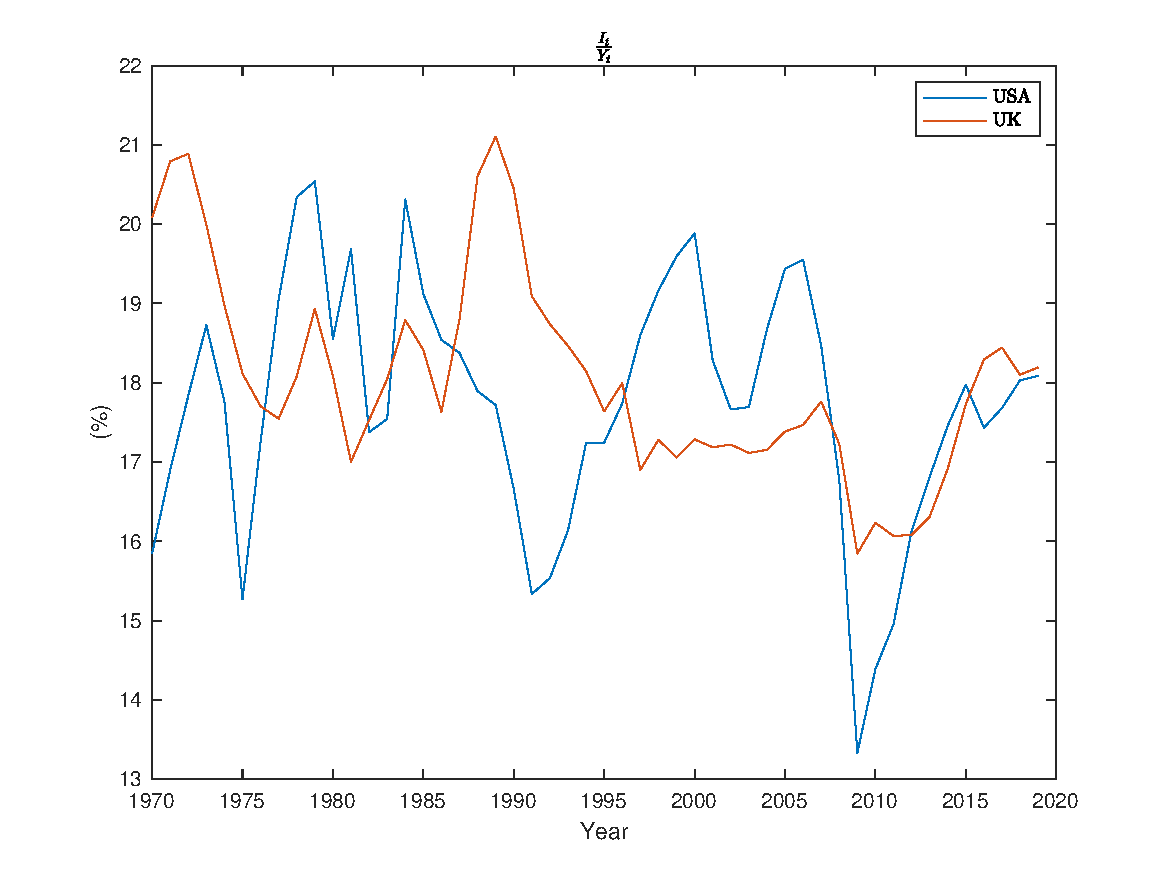
\includegraphics[width=0.7\textwidth]{out/Investment.pdf}
    \centering
    \caption{Investment-GDP ratio comparison}
\end{figure}

The US investment to GDP ratio has fluctuated between $\sim 13.3\% $ and $20.5\%$ between 1970 and 2019 while the UK investment to GDP ratio has fluctuated between $15.8\%$ to $21.1\%$ in the same period. However, US investment to GDP ratio has shown more volality (as measured by long-run standard deviation) compared to UK.
\\
\\
% QUESTION 1 ENDS HERE

%%%%%%%%%%%%%%%%%%%%%%%%%%%%%%%%%%%%%%%%%%%%%%%%%%%%%%%%%%%%%%%%%%%%

2. \textbf{Use the real investment series, the capital accumulation equation}
$$
K_{t+1}=(1-\delta) K_t+I_t
$$

and follow the numerical method we discussed in class to jointly determine the values of $\delta, K_0$, and $\left\{K_t\right\}_{t=1}^T$. Specifically, you will choose the initial capital stock to satisfy

$$
\frac{K_0}{Y_0}=\left(\frac{1}{10}\right)\left(\sum_{t=1}^{10}\left(K_t / Y_t\right)\right)
$$

\noindent given data on initial real GDP, and GDP for the following 10 periods. You will choose the depreciation rate such that sample average depreciation expenditure as a portion of GDP calculated in the data using each country's National Income and Product Accounts (NIPA) data equals that implied by the sample average product of your constructed (real) capital stock and depreciation rate as a ratio of (real) GDP. And use the capital accumulation equation to calculate the time-series of capital stocks over your sample period. You should not use independent sources of information on the depreciation rate, or initial capital stock in making these calculations.
\\ \\ 
\textbf{Answer}: I use numerical optimization on MATLAB (\textit{fsolve}) to jointly determine the values of $\delta, K_0$, and $\left\{K_t\right\}_{t=1}^T$ between 1970 and 2019. 

% Please add the following required packages to your document preamble:
% \usepackage{booktabs}
\begin{table}[h]
    \centering
    \caption{$K_0$ value }
    \label{tab:table-1}
    \begin{tabular}{@{}lcc@{}}
    \toprule
    Country & Arithmetic mean (n=10) & $\delta$ \\ \midrule
    United States & 9.7794 & 0.0682 \\
    United Kingdom & 0.1482 & 0.1056
    \end{tabular}
    \end{table}

UK has a higher rate of depreciation than US.
\\ \\ 
3. \textbf{Repeat part 2. using a geometric ten-year average of capital-output ratios in the initial capital stock formula}, rather than a simple arithmetic average, and compare the two capital stock series you have constructed for each country by plotting them and calculating
\begin{itemize}
    \item their simple correlation,
    \item their relative standard deviations,
    \item their relative growth rates.
\end{itemize}

Discuss how and why they differ.
\\ \\
By the AM-GM inequality, we know that the geometric mean would be lesser than the arithmetic mean.

% Please add the following required packages to your document preamble:
% \usepackage{booktabs}
\begin{table}[h]
    \centering
    \caption{$K_0$ value }
    \label{tab:table-1}
    \begin{tabular}{@{}lccc@{}}
    \toprule
    Country & Geometric mean (n=10) & Arithmetic mean (n=10) & $\delta$ \\ \midrule
    United States & 9.5187 & 9.7794 & 0.0682 \\
    United Kingdom & 0.1475 & 0.1482 & 0.1056 \\ \bottomrule
    \end{tabular}
    \end{table}

Additionally, we are required to calculate the correlation between the 10-year arithmetic and geometric mean as well as the relative standard deviation and growth rates. 

\begin{table}[h]
    \centering
    \caption{Comparison of Capital series for US}
    \label{tab:US_K}
    \begin{tabular}{@{}lll@{}}
    \toprule
    Moment & Arithmetic mean (n=10) & Geometric mean (n=10) \\ \midrule
    Correlation & 1 & 0.99999 \\
    Relative SD & 1 & 1.0065 \\
    Average growth rate & 1 & 1.019 \\ \bottomrule
    \end{tabular}
    \end{table}

\begin{table}[h]
    \centering
    \caption{Comparison of Capital series for UK}
    \label{tab:UK_K}
    \begin{tabular}{@{}lll@{}}
    \toprule
    Moment & Arithmetic mean (n=10) & Geometric mean (n=10) \\ \midrule
    Correlation & 1 & 1 \\
    Relative SD & 1 & 1.003 \\
    Average growth rate & 1 & 1.0048 \\ \bottomrule
    \end{tabular}
    \end{table}

I now plot the capital series for each country.

\begin{figure}
    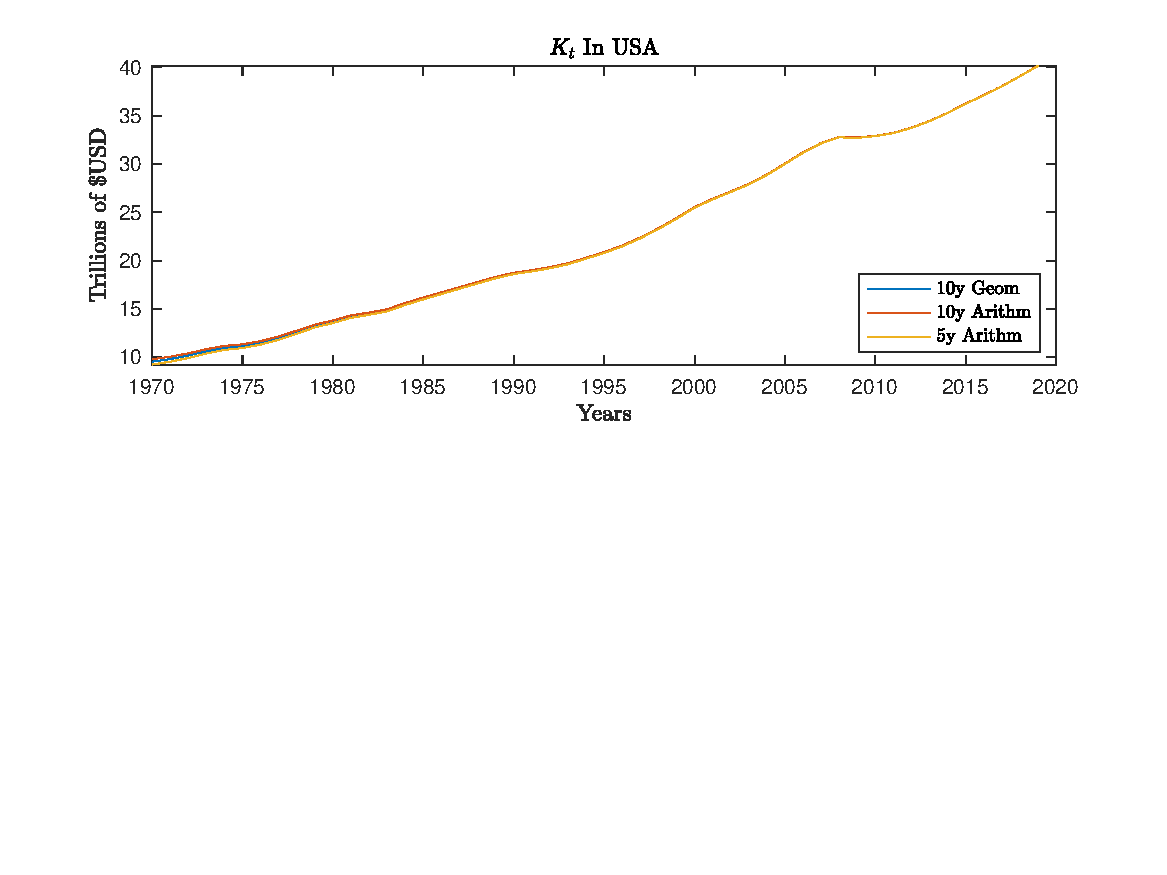
\includegraphics[trim = 0in 3.2in 0in 0in, clip, width=1\textwidth]{out/Capital_Series_US.pdf}
    \caption{Capital series for US}
\end{figure}

\begin{figure}[h]
    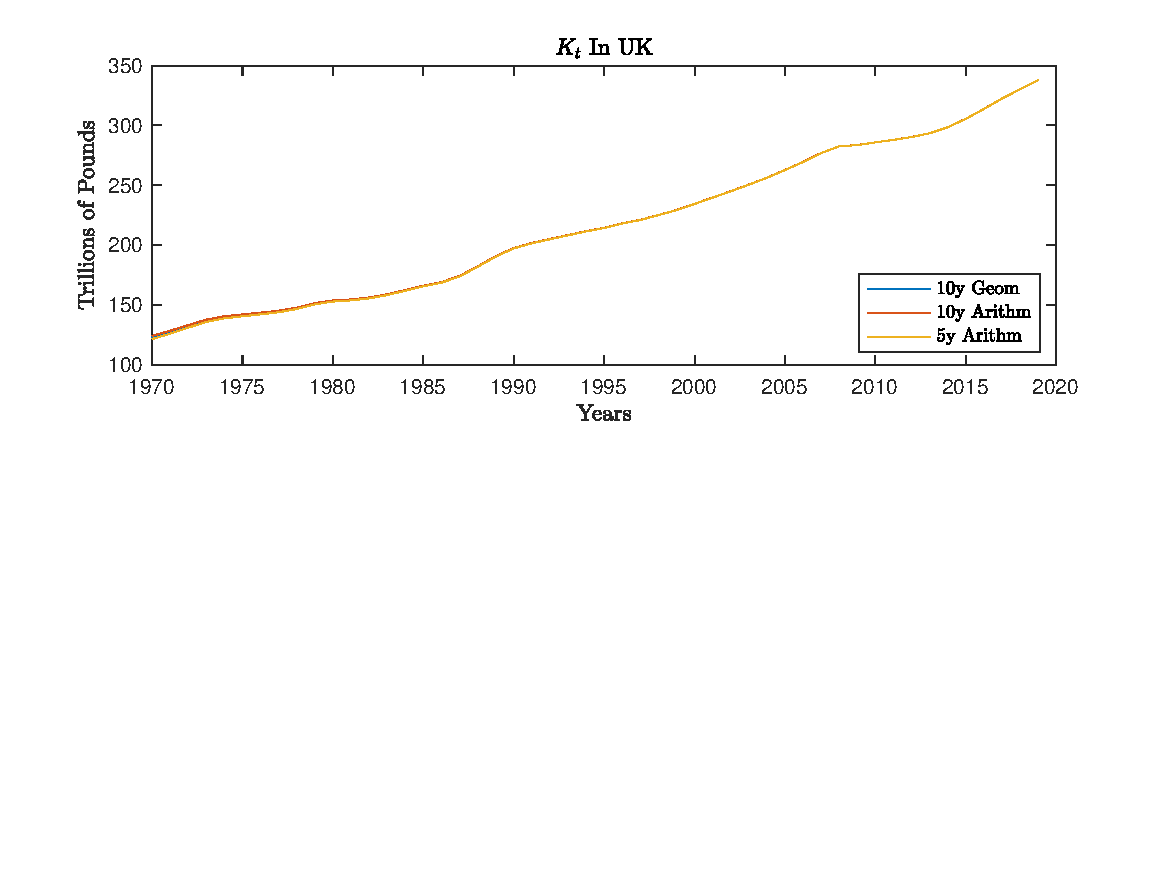
\includegraphics[trim = 0in 3.2in 0in 0in, clip, width=1\textwidth]{out/Capital_Series_uk.pdf}
    \caption{Capital series for UK}
\end{figure}

Note that the differences in the capital stock series constructed using the capital accumulation equation have very minimal differences which suggests that the estimates are robust to the method employed. 
\\ \\
4. \textbf{Repeat part 2 using the five-year arithmetic mean of capital-output ratios after the initial period rather than 10-year arithmetic mean to calculate the initial capital stock}. Does this matter, quantitatively, for the capital stock series you compute for each country? Again, plot the two series and compare their statistical properties (first and second moments).
\\ \\ 
\textbf{Answer:} I repeat the same exercise for both countries using 5-year and 10-year averages. The plots above also show the 5-year series, which is nearly identical to the 10-year arithmetic mean and 10-year geometric mean capital stock series. 
\\ \\ 
I show the show the statistical properties of the 5-year arithmetic average capital stock series.

% Please add the following required packages to your document preamble:
% \usepackage{booktabs}
\begin{table}[h]
    \centering
    \caption{Comparison of Capital series for the US with 5-year arithmetic average}
    \label{tab:US_K_2}
    \begin{tabular}{@{}llll@{}}
    \toprule
    Moment & \begin{tabular}[c]{@{}l@{}}Arithmetic \\ mean (n=10)\end{tabular} & \begin{tabular}[c]{@{}l@{}}Geometric \\ mean (n=10)\end{tabular} & \begin{tabular}[c]{@{}l@{}}Arithmetic \\ mean (n=5)\end{tabular} \\ \midrule
    Correlation & 1 & 0.99999 & 0.99997 \\
    Relative SD & 1 & 1.0065 & 1.0139 \\
    Average growth rate & 1 & 1.019 & 1.041 \\ \bottomrule
    \end{tabular}
    \end{table}

\begin{table}[h]
    \centering
    \caption{Comparison of Capital series for UK with 5-year arithmetic average}
    \label{tab:UK_K_2}
    \begin{tabular}{@{}llll@{}}
    \toprule
    Moment & \begin{tabular}[c]{@{}l@{}}Arithmetic \\ mean (n=10)\end{tabular} & \begin{tabular}[c]{@{}l@{}}Geometric \\ mean (n=10)\end{tabular} & \begin{tabular}[c]{@{}l@{}}Arithmetic \\ mean (n=5)\end{tabular} \\ \midrule
    Correlation & 1 & 1 & 0.99986 \\
    Relative SD & 1 & 1.003 & 0.99656 \\
    Average growth rate & 1 & 1.0048 & 0.94215 \\ \bottomrule
    \end{tabular}
    \end{table}

Similar to part 3, we see that the correlation between the 10-year and 5-year arithmetic average is near-perfect, indicating the robustness of the capital stock estimates.
\\ \\ 
5. \textbf{If there are capital stock series available online for your three countries, for example the PPP series in the Penn World Tables or the nominal series in the IMF’s capital and investment dataset, compare your constructed series for each country to the published series and try to uncover any reasons for the differences}. Again, plot the series against one another and compare their first and second moments.
\\ \\ 
\textbf{Answer}: I use data from the Penn World Tables (v10.01), running from 1950 to 2019. I now plot comparison of the capital stock series for each country against their corresponding PWT capital stock series.

\begin{figure}
    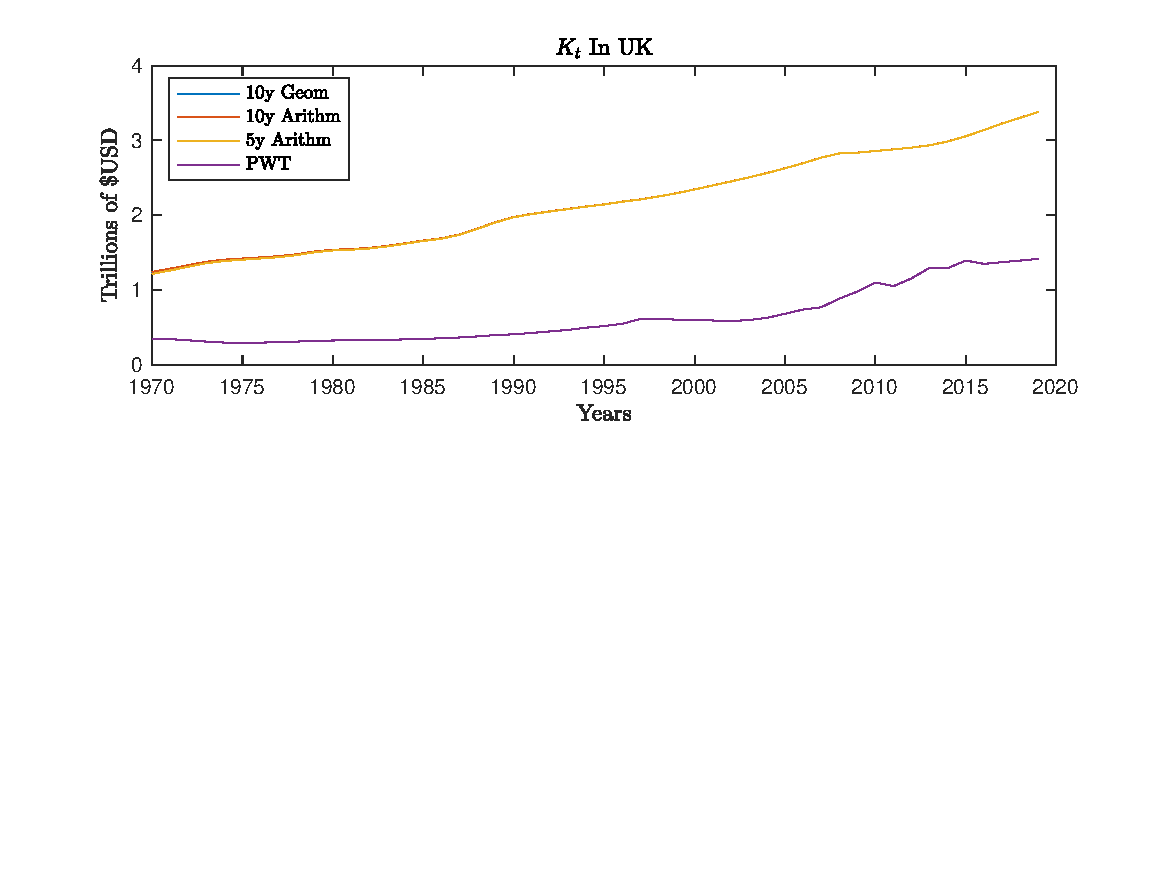
\includegraphics[trim = 0in 3.2in 0in 0in, clip, width=1\textwidth]{out/Capital_Series_PWT_UK.pdf}
    \caption{Capital series for UK}
\end{figure}

\begin{figure}[]
    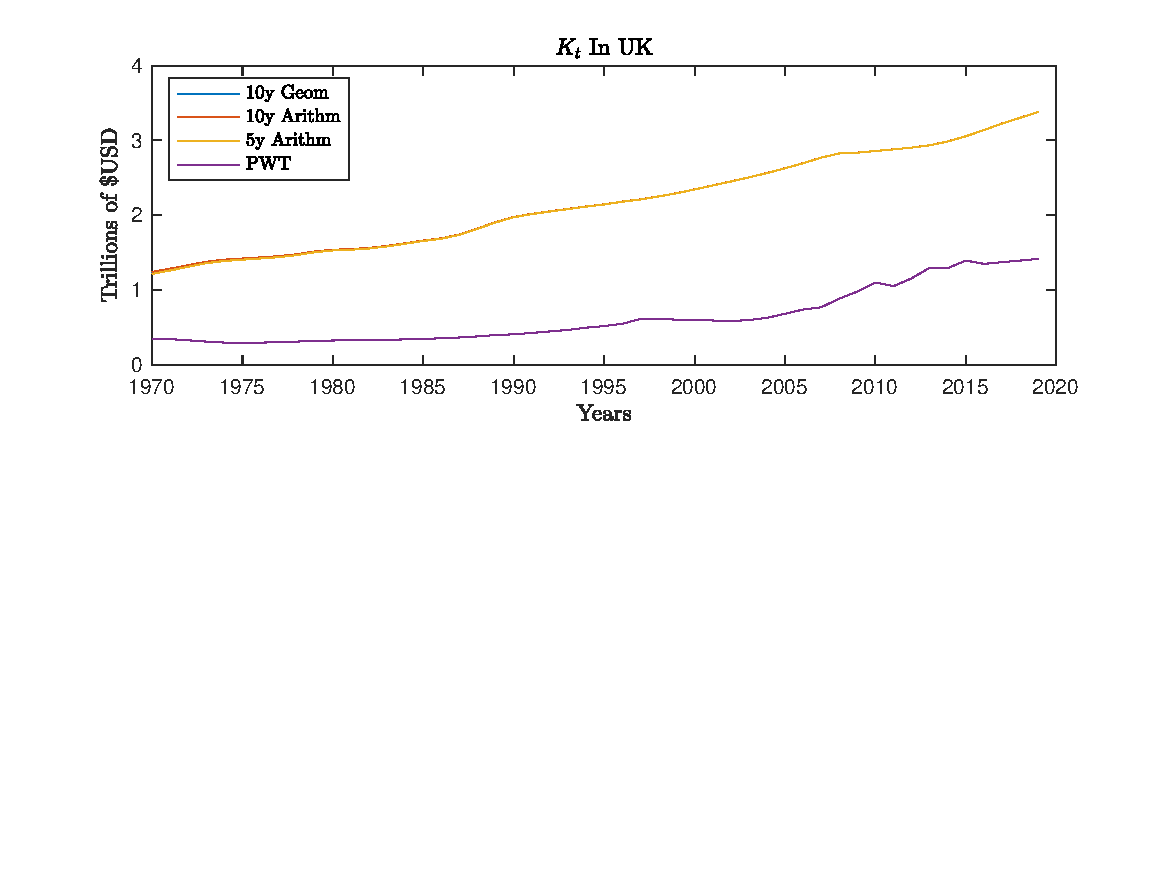
\includegraphics[trim = 0in 3.2in 0in 0in, clip, width=1\textwidth]{out/Capital_Series_PWT_UK.pdf}
    \caption{Capital series for UK}
\end{figure}
\end{document}